\documentclass[conference]{IEEEtran}
\IEEEoverridecommandlockouts
\usepackage{cite}
\usepackage{amsmath,amssymb,amsfonts}
\usepackage{algorithmic}
\usepackage{graphicx}
\usepackage{textcomp}
\usepackage{xcolor}
\def\BibTeX{{\rm B\kern-.05em{\sc i\kern-.025em b}\kern-.08em
    T\kern-.1667em\lower.7ex\hbox{E}\kern-.125emX}}

\begin{document}

\title{Evaluating Feature-Pruned Cross-Network Transfer, Class-Conditional Mondrian Calibration, and Selective Routing in Network Intrusion Detection}

\author{\IEEEauthorblockN{Shreyas Gautam}
\IEEEauthorblockA{\textit{Department of Computer Science and Engineering} \\
\textit{Chandigarh University}\\
Mohali, Punjab, India \\
gautamshreyas4@gmail.com}
}

\maketitle

\begin{abstract}
Machine learning-based Network Intrusion Detection Systems (ML-NIDS) routinely achieve high closed-set F1-scores on single-environment splits while failing under cross-network transfer, severe class imbalance, and previously unseen attack families. Rather than claiming a universally domain-invariant classifier, this paper presents an empirical reliability audit and integration study investigating how progressive header-feature pruning, coupled volumetric monotonicity, calibration-fitted open-set extreme value modeling, class-conditional Mondrian conformal prediction, and validation-tuned selective routing interact across standardized NetFlow v2 benchmarks (NF-UNSW-NB15-v2 and NF-CSE-CIC-IDS2018-v2). First, post-split deduplication strictly within the proper training partition reveals that under a 30-feature behavioral schema (Set C), 95.23 percent of training records collapse into identical feature projections. Second, across 32 directional cross-dataset model fits with a fixed target sample seed, removing Time-To-Live (TTL) alone (Set A) triggers a non-monotonic shortcut cascade where decision trees overfit unpruned TCP window and protocol identifiers (forward Macro-F1 dropping from 0.4499 to 0.3992), whereas pruning all three header groups (Set C) recovers transfer above baseline in both forward (0.4549) and reverse (0.4756 vs. 0.4701) directions, though absolute cross-network Balanced Accuracy remains near random chance (0.4634 to 0.4703). Third, on the unified full test split (297,988 known-class flows and 164 withheld Worms flows), standard marginal split conformal prediction at 90 percent target coverage achieves 90.40 percent aggregate coverage by covering 96.07 percent of benign flows while collapsing to 0.00 percent coverage on Analysis, Reconnaissance, and Shellcode attacks (mean class coverage 18.96 percent). Unpooled class-conditional Mondrian calibration restores worst-class empirical coverage to 86.94 percent and mean class coverage to 90.46 percent. Finally, a validation-tuned selective routing gate automates 85.35 percent of test traffic at 99.50 percent overall accuracy (93.29 percent attack-only accuracy) and escalates 98.78 percent (162 of 164 flows) of unseen Worms attacks (31.71 percent via open-set rejection and 67.07 percent via conformal ambiguity), reducing gate-consistent cumulative risk to 0.0124.
\end{abstract}

\begin{IEEEkeywords}
network intrusion detection, cross-dataset generalization, shortcut learning, Mondrian conformal prediction, open-set recognition, selective classification
\end{IEEEkeywords}

\section{Introduction}
Machine learning classifiers evaluated on single-network intrusion detection benchmarks frequently report closed-set F1-scores exceeding 99\% \cite{b1,b2}. Independent forensic audits have established that these figures are often inflated by extraction defects in legacy flow generators, testbed-specific shortcut learning, and evaluation protocols that ignore operational base-rate skew \cite{b1,b3,b4,b5}. When models trained on one network capture are evaluated zero-shot on a distinct network environment, classification performance frequently degrades toward random guessing \cite{b6,b7}. Furthermore, in operational Security Operations Centers (SOCs), benign background traffic outnumbers malicious flows by one to three orders of magnitude \cite{b2}. Under such severe class imbalance, uncalibrated classifiers and marginal uncertainty wrappers either overwhelm human analysts with false alarms or silently misclassify rare and previously unseen attack families \cite{b1,b8}.

Recent literature has examined individual components of NIDS reliability, including cross-dataset generalization studies \cite{b6,b7}, open-set intrusion recognition via Extreme Value Theory (EVT) \cite{b9,b10}, and conformal prediction with reject options \cite{b11,b12,b13}. However, a critical empirical gap remains in understanding how these mechanisms interact—and where their theoretical assumptions break down—when integrated into a unified flow-processing architecture. Specifically, this study investigates three concrete research questions:
\begin{enumerate}
    \item \textit{Shortcut Cascade vs.\ Domain Transfer:} When environment-coupled packet header attributes (Time-To-Live, TCP window sizes, and protocol identifiers) are progressively removed under post-split training deduplication, does cross-network generalization improve monotonically, or do decision trees shift reliance onto secondary header shortcuts before recovering?
    \item \textit{Full-Scale Marginal Collapse vs.\ Mondrian Restoration:} On an un-subsampled test distribution where benign traffic constitutes over 92\% of flows, how severely does standard Marginal Split Conformal Prediction (SCP) starve minority attack categories of coverage, and how effectively does unpooled Class-Conditional Mondrian Conformal Prediction (MCP) equalize per-class coverage?
    \item \textit{Complementary Deferral of Withheld Attack Families:} How do calibration-fitted Mahalanobis EVT rejection and Mondrian conformal set ambiguity complement one another when routing unseen attack families between automated resolution and human analyst review?
\end{enumerate}

Rather than claiming a universally topology-invariant classifier or an unconditional conformal guarantee under temporal drift, this paper contributes a rigorously unified empirical audit across `NF-UNSW-NB15-v2` and `NF-CSE-CIC-IDS2018-v2` \cite{b2}, evaluating Open-Set Recognition (Suite E3), Mondrian Conformal Prediction (Suite E4), and Selective SOC Routing (Suite E5a) on the exact same full-scale test population ($N_{\text{test}} = 298,152$ flows).

\section{Data Provenance, Feature Projection Redundancy, and Partitioning}

\subsection{Pre-Cleaned NetFlow v2 Parquet Snapshots}
Raw CSV releases of `CIC-IDS2017` and `CSE-CIC-IDS2018` extracted via `CICFlowMeter` suffer from documented TCP termination bugs, negative flow durations, and 6.67\% to 7.53\% label corruption \cite{b3,b4,b5}. To evaluate cross-network transfer across a standardized schema without `CICFlowMeter` extraction artifacts, we ingest pre-cleaned Parquet snapshots of the University of Queensland NetFlow v2 (`NF-v2`) benchmarks: `NF-UNSW-NB15-v2` and `NF-CSE-CIC-IDS2018-v2` \cite{b2}.

Table~\ref{tab:dataset_provenance} reconciles the published raw UQ flow counts \cite{b2} against the ingested Kaggle Parquet snapshots (`dhoogla/nfunswnb15v2` and `dhoogla/nfcsecicids2018v2`). Upstream Parquet conversion removed raw IP string columns (`IPV4_SRC_ADDR`, `IPV4_DST_ADDR`) and exact 43-column duplicates, yielding 1,986,745 zero-null flows in `NF-UNSW-NB15-v2` ($-16.88\%$ vs.\ raw UQ) and 17,129,715 zero-null flows in `NF-CSE-CIC-IDS2018-v2` ($-9.34\%$ vs.\ raw UQ). Each dataset contains 43 total columns: 41 shared numerical flow attributes, binary `Label` ($\{0, 1\}$), and multi-class `Attack`.

\begin{table}[t]
\caption{Reconciliation of Published UQ NetFlow v2 Releases vs.\ Ingested Pre-Cleaned Parquet Snapshots}
\begin{center}
\begin{tabular}{|l|r|r|}
\hline
\textbf{Dataset Property} & \textbf{NF-UNSW-NB15-v2} & \textbf{NF-CSE-CIC-IDS2018-v2} \\
\hline
Published UQ Raw Flows \cite{b2} & 2,390,275 & 18,893,708 \\
Upstream Duplicate/IP Drop & $-403,530$ ($-16.88\%$) & $-1,763,993$ ($-9.34\%$) \\
\textbf{Ingested Parquet Flows} & \textbf{1,986,745} & \textbf{17,129,715} \\
\hline
Total Parquet Columns & 43 & 43 \\
Shared Numerical Attributes & 41 & 41 \\
Null / Missing Cells & 0 & 0 \\
\hline
Benign Flows (\texttt{Label = 0}) & 1,911,666 (96.22\%) & 15,101,685 (88.16\%) \\
Attack Flows (\texttt{Label = 1}) & 75,079 (3.78\%) & 2,028,030 (11.84\%) \\
Binary Imbalance Ratio & $25.46 : 1$ & $7.45 : 1$ \\
\hline
\end{tabular}
\label{tab:dataset_provenance}
\end{center}
\end{table}

\subsection{Overflow Sanitization and Progressive Feature Pruning}
In `NF-CSE-CIC-IDS2018-v2`, sub-millisecond burst calculations in `float64` byte-rate columns (`SRC_TO_DST_SECOND_BYTES`, `DST_TO_SRC_SECOND_BYTES`) exceed the maximum finite 32-bit float ($\approx 3.40 \times 10^{38}$). Our `ForensicDataSanitizer` clamps all numerical features to $[-10^{15}, 10^{15}]$ before casting to `float32` and verifies zero negative durations or zero-packet flows (`Dropped_Negative_Duration = 0`, `Dropped_Zero_Packets = 0`, retaining all 1,986,745 rows).

To investigate shortcut learning across header groups \cite{b1,b6}, we strip explicit port numbers (`L4_SRC_PORT`, `L4_DST_PORT`) from the 41 numerical columns and define four nested feature schemas:
\begin{itemize}
    \item \textbf{Baseline Schema (39 features):} Drops `L4_SRC_PORT` and `L4_DST_PORT`, retaining all 39 remaining numerical attributes.
    \item \textbf{Set A (37 features):} Additionally drops Time-To-Live fields (`MIN_TTL`, `MAX_TTL`).
    \item \textbf{Set B (35 features):} Additionally drops TCP window size fields (`TCP_WIN_MAX_IN`, `TCP_WIN_MAX_OUT`).
    \item \textbf{Set C (30 features):} Additionally drops 5 protocol and query/type identifier fields (`PROTOCOL`, `L7_PROTO`, `ICMP_TYPE`, `ICMP_IPV4_TYPE`, `DNS_QUERY_ID`), retaining 30 pure behavioral volume, rate, duration, and retransmission features.
\end{itemize}

\subsection{Global Sequential Partitioning and Post-Split Training Deduplication}
Because the pre-cleaned Parquet snapshots omit raw capture timestamps, `create_temporal_four_way_split()` partitions all $1,986,581$ known-class flows ($\mathcal{Y}_{\text{known}} = \{0, \dots, 8\}$) across global sequential row cutoffs into four disjoint subsets: Proper Training $Z_t$ ($55\%$, $1,092,619$ initial rows), Validation $Z_v$ ($15\%$, $297,987$ rows), Calibration $Z_c$ ($15\%$, $297,987$ rows), and Locked Known Evaluation $Z_{\text{test, known}}$ ($15\%$, $297,988$ rows). Every known class satisfies minimum support across the global cutoffs (`Localized_Campaign_Fallbacks = 0`). The withheld `Worms` category ($164$ flows, mapped to label $-1$) is excluded from $Z_t, Z_v,$ and $Z_c$ and appended strictly to the test split, yielding $N_{\text{test}} = 298,152$ total test flows.

Crucially, to prevent duplicate-induced training bias while strictly preserving the natural test distribution \cite{b1}, exact feature-vector deduplication is performed **exclusively on $Z_t$ after splitting**. Under the 30-feature `Set_C` projection, removing port, TTL, window, and protocol headers causes $1,040,482$ of the $1,092,619$ training rows ($95.23\%$) to collapse into identical 30-dimensional feature-label pairs, leaving $52,137$ unique training patterns in $Z_t$ while keeping $Z_v, Z_c,$ and $Z_{\text{test}}$ completely unaltered. A `RobustScaler` is fitted solely on the deduplicated $Z_t$ and applied to $Z_v, Z_c,$ and $Z_{\text{test}}$.

\section{Methodology and Mathematical Formulation}

\subsection{Coupled Binary-Monotone and Multiclass GBDT Backbone}
Tree ensembles consistently outperform deep neural architectures on tabular data with irregular decision boundaries \cite{b14}. However, standard `scikit-learn` `HistGradientBoostingClassifier` supports monotonic constraints (`monotonic_cst`) only for binary and regression targets, disabling them when $K > 2$. To preserve volumetric monotonicity across our 9-class pipeline, `HybridNIDSBackbone` couples two gradient-boosted ensembles trained on $Z_t$ (each with 200 max iterations, 63 leaf nodes, learning rate $0.08$, and balanced class weights):
\begin{enumerate}
    \item \textit{Binary Monotone Gate ($h_{\text{mono}}$):} Trained on binary labels $y_{\text{bin}} = \mathbb{I}[y > 0] \in \{0, 1\}$ with constraint vector $m_j = +1$ for all volumetric/rate features $j \in \mathcal{F}_{\text{vol}}$ (columns containing `BYTES`, `PKTS`, or `THROUGHPUT`) and $m_j = 0$ otherwise \cite{b15}. For any $\mathbf{x}, \mathbf{x}' \in \mathbb{R}^d$ satisfying $x_j \le x'_j \; \forall j \in \mathcal{F}_{\text{vol}}$ and $x_j = x'_j \; \forall j \notin \mathcal{F}_{\text{vol}}$:
    \begin{equation}
    f_{\text{mono}}(\mathbf{x}) \le f_{\text{mono}}(\mathbf{x}') \implies \hat{P}_{\text{mono}}(Y > 0 \mid \mathbf{x}) \le \hat{P}_{\text{mono}}(Y > 0 \mid \mathbf{x}').
    \label{eq:mono_bin}
    \end{equation}
    \item \textit{Multiclass Specialist ($h_{\text{multi}}$):} Trained on $y \in \{0, \dots, K-1\}$ to estimate class probabilities $\hat{P}_{\text{multi}}(Y = c \mid \mathbf{x})$.
\end{enumerate}
At inference, the coupled $K$-class probability distribution $\hat{P}_h(Y = c \mid \mathbf{x})$ is constructed via exact probability factorization:
\begin{align}
\hat{P}_h(Y = 0 \mid \mathbf{x}) &= 1 - \hat{P}_{\text{mono}}(Y > 0 \mid \mathbf{x}), \label{eq:coupled_0} \\
\hat{P}_h(Y = c \mid \mathbf{x}) &= \hat{P}_{\text{mono}}(Y > 0 \mid \mathbf{x}) \cdot \frac{\hat{P}_{\text{multi}}(Y = c \mid \mathbf{x})}{\sum_{j=1}^{K-1} \hat{P}_{\text{multi}}(Y = j \mid \mathbf{x})}, \;\; c \ge 1.
\label{eq:coupled_c}
\end{align}
By (\ref{eq:mono_bin})--(\ref{eq:coupled_c}), $\sum_{c=0}^{K-1} \hat{P}_h(Y = c \mid \mathbf{x}) = 1$, and increasing any volumetric feature $x_j \in \mathcal{F}_{\text{vol}}$ is guaranteed never to increase benign probability $\hat{P}_h(Y = 0 \mid \mathbf{x})$ or decrease total attack probability $\sum_{c=1}^{K-1} \hat{P}_h(Y = c \mid \mathbf{x})$.

\subsection{Calibration-Fitted Open-Set Recognition (Mahalanobis EVT + PCA)}
To detect unknown attack families ($\mathcal{Y}_{\text{unknown}} = \{-1\}$), `DualStageOpenSetDetector` operates on the joint feature-and-margin representation $\mathbf{v}(\mathbf{x}) = [\mathbf{x}_{\text{scaled}}, \mathbf{g}(\mathbf{x})] \in \mathbb{R}^{d+K}$, where $\mathbf{g}(\mathbf{x}) \in \mathbb{R}^K$ denotes the raw decision margins of $h_{\text{multi}}$.

For each known class $c \in \mathcal{Y}_{\text{known}}$, we estimate the class centroid $\boldsymbol{\mu}_c \in \mathbb{R}^{d+K}$, regularized inverse covariance matrix $\boldsymbol{\Sigma}_c^{+} = (\text{Cov}(V_{t,c}^{+}) + 10^{-3}\mathbf{I}_{d+K})^{+}$, and $d_{\text{pca}} = \min(16, |Z_{t,c}^{+}|-1, d+K-1)$ Principal Component Analysis (PCA) subspace projector $\mathcal{P}_c$ on correctly classified training instances $Z_{t,c}^{+}$. For any representation $\mathbf{v}(\mathbf{x})$, the class-conditional Mahalanobis distance is:
\begin{equation}
d_M(\mathbf{v}(\mathbf{x}), c) = \sqrt{\max\left(10^{-12}, \; (\mathbf{v}(\mathbf{x}) - \boldsymbol{\mu}_c)^\top \boldsymbol{\Sigma}_c^{+} (\mathbf{v}(\mathbf{x}) - \boldsymbol{\mu}_c)\right)}.
\label{eq:maha}
\end{equation}
To prevent in-sample GBDT margin compression on $Z_t$ from causing excessive false rejections at test time, we fit the two-parameter Weibull tail distribution $W_c(d) = 1 - \exp(-(d/\lambda_c)^{\kappa_c})$ (via maximum likelihood on the $\eta = 50$ largest distances) and the 98th-percentile PCA reconstruction error threshold $\theta_c = Q_{0.98}(\{\mathcal{L}_{\text{rec}}(\mathbf{x}_i; c)\})$ on the **held-out calibration stratum $Z_{c,c}$** (`cal_fallback_classes = 0`).

Furthermore, rather than attenuating shifted logits (which falsely transfers mass from non-predicted classes), we apply Weibull attenuation directly in probability space over $\mathbf{p}(\mathbf{x}) = \text{Softmax}(\mathbf{g}(\mathbf{x}))$:
\begin{align}
\tilde{p}_c(\mathbf{x}) &= p_c(\mathbf{x}) \cdot \left(1 - \vartheta W_c(d_M(\mathbf{v}(\mathbf{x}), c))\right), \label{eq:prob_atten} \\
m_{\text{trans}}(\mathbf{x}) &= \sum_{c=0}^{K-1} \left(p_c(\mathbf{x}) - \tilde{p}_c(\mathbf{x})\right) = \vartheta \sum_{c=0}^{K-1} p_c(\mathbf{x}) W_c(d_M(\mathbf{v}(\mathbf{x}), c)). \label{eq:trans_mass}
\end{align}
Letting $\hat{c} = \arg\max_{c} p_c(\mathbf{x})$ and $r_{\text{rec}}(\mathbf{x}) = \mathcal{L}_{\text{rec}}(\mathbf{x}; \hat{c}) / \theta_{\hat{c}}$ denote the normalized subspace reconstruction ratio, the continuous open-set score combines base margin uncertainty, Weibull tail mass transfer, and subspace excess:
\begin{align}
s_{\text{OSR}}(\mathbf{x}) &= 0.40 \left(1 - \max_c p_c(\mathbf{x})\right) + 0.40 \, m_{\text{trans}}(\mathbf{x}) \nonumber \\
&\quad + 0.20 \left(1 - \exp(-\max(0, r_{\text{rec}}(\mathbf{x}) - 1))\right).
\label{eq:osr_score}
\end{align}
The binary open-set rejection gate is $R_{\text{OSR}}(\mathbf{x}) = \mathbb{I}[s_{\text{OSR}}(\mathbf{x}) > \tau_{\text{OSR}}] \lor \mathbb{I}[r_{\text{rec}}(\mathbf{x}) > 1]$, where $\tau_{\text{OSR}} = Q_{0.97}(\{s_{\text{OSR}}(\mathbf{x}_i) : \mathbf{x}_i \in Z_v\})$ is calibrated on the validation partition $Z_v$ to cap false rejection on known validation traffic.

\subsection{Inductive Class-Conditional (Mondrian) Conformal Prediction}
Given calibration partition $Z_c$, `MondrianConformalCalibrator` partitions $Z_c$ by true label $\tilde{y} \in \mathcal{Y}_{\text{known}}$ into $K = 9$ strata $Z_{c,\tilde{y}}$ of size $n_{\tilde{y}}$ with nonconformity scores $s_i^{(\tilde{y})} = 1 - \hat{P}_h(Y = \tilde{y} \mid \mathbf{x}_i)$ \cite{b8,b16}. As verified in Table~\ref{tab:e4_per_class}, the smallest calibration stratum in `NF-UNSW-NB15-v2` is `Analysis` with $n_{\tilde{y}} = 154$ flows, followed by `Backdoor` ($n_{\tilde{y}} = 170$) and `Shellcode` ($n_{\tilde{y}} = 421$). Because $154 \ge 19 = \lceil (1-0.05)/0.05 \rceil$, **zero classes ($0/9$) activate nearest-stratum KS pooling**; every class is calibrated strictly on its own unpooled calibration stratum.

Sorting $S_{\tilde{y}} = \{s_1^{(\tilde{y})} \le \dots \le s_{n_{\tilde{y}}}^{(\tilde{y})}\}$ once during fitting allows `compute_mondrian_p_values()` to evaluate tie boundaries within $\epsilon = 10^{-7}$ for $s_{\text{test}} = 1 - \hat{P}_h(Y = \tilde{y} \mid \mathbf{x}_{\text{test}})$ via $\mathcal{O}(K N_{\text{test}} \log n_{\tilde{y}})$ binary search (`np.searchsorted`), using $4.55\text{ MiB}$ of working index-buffer memory and $20.47\text{ MiB}$ for the returned $N_{\text{test}} \times K$ `float64` p-value matrix (compared to $79.59\text{ GiB}$ for naive 2D broadcasting):
\begin{align}
p_{\tilde{y}}(\mathbf{x}_{\text{test}}) &= \frac{\left|\{i \in Z_{c,\tilde{y}} : s_i^{(\tilde{y})} > s_{\text{test}} + \epsilon\}\right|}{n_{\tilde{y}} + 1} \nonumber \\
&\quad + \frac{\theta \left(\left|\{i \in Z_{c,\tilde{y}} : |s_i^{(\tilde{y})} - s_{\text{test}}| \le \epsilon\}\right| + 1\right)}{n_{\tilde{y}} + 1},
\label{eq:mondrian_pval}
\end{align}
where $\theta \sim \text{Uniform}[0, 1]$ \cite{b16}. The prediction set at miscoverage level $\alpha$ is $\Gamma^\alpha(\mathbf{x}_{\text{test}}) = \{\tilde{y} \in \mathcal{Y}_{\text{known}} : p_{\tilde{y}}(\mathbf{x}_{\text{test}}) > \alpha\}$. Because sequential row-order partitioning across network capture periods does not guarantee strict exchangeability between $Z_c$ and $Z_{\text{test}}$ \cite{b19,b20}, we evaluate coverage as an empirical measurement against the nominal $(1-\alpha)$ target.

\subsection{Validation-Tuned Selective Routing and Gate-Consistent AURC}
Let $p_{(1)}(\mathbf{x}) \ge p_{(2)}(\mathbf{x})$ denote the two largest Mondrian p-values for flow $\mathbf{x}$, and define the conformal evidence-margin ranking heuristic $\delta^{\text{em}}(\mathbf{x}) = p_{(1)}(\mathbf{x}) - p_{(2)}(\mathbf{x})$. `SOCTriageEngine` assigns final prediction $\hat{y}_{\text{final}}(\mathbf{x}) = -1$ if $R_{\text{OSR}}(\mathbf{x}) = 1$ else $\arg\max_{c} \hat{P}_h(Y = c \mid \mathbf{x})$, and routes $\mathbf{x}$ to the \textbf{Automated Resolution Queue ($\mathcal{A}$)} if and only if:
\begin{equation}
\mathbf{x} \in \mathcal{A} \iff \left(|\Gamma^\alpha(\mathbf{x})| = 1\right) \land \left(\neg R_{\text{OSR}}(\mathbf{x})\right) \land \left(\delta^{\text{em}}(\mathbf{x}) \ge \tau_{\text{hi}}\right).
\label{eq:triage_gate}
\end{equation}
All other flows are deferred to the \textbf{Escalated Analyst Queue ($\mathcal{E} = Z_{\text{test}} \setminus \mathcal{A}$)}. Rather than hardcoding $\tau_{\text{hi}}$ on test data, `tune_threshold_on_validation()` sweeps $\tau \in [0.05, 0.50]$ on the validation split $Z_v$ to minimize the operational cost function:
\begin{equation}
\mathcal{L}_{\text{SOC}}(\tau) = C_{\text{FN}} N_{\text{FN, auto}}(\tau) + C_{\text{FP}} N_{\text{FP, auto}}(\tau) + C_{\text{E}} N_{\text{Escalated}}(\tau),
\label{eq:soc_cost}
\end{equation}
with $C_{\text{FN}} = 10, C_{\text{FP}} = 2, C_{\text{E}} = 1$, selecting $\tau_{\text{hi}} = 0.0500$ on $Z_v$.

To evaluate selective ranking consistently with the gate conditions in (\ref{eq:triage_gate}), we define the gate-consistent priority score $\pi(\mathbf{x}) = 10 \cdot \mathbb{I}[|\Gamma^\alpha(\mathbf{x})| = 1 \land \neg R_{\text{OSR}}(\mathbf{x})] + \delta^{\text{em}}(\mathbf{x})$ (which orders singleton non-rejected flows ahead of escalated flows) and compute both standalone margin $\text{AURC}_{\text{margin}}$ and $\text{AURC}_{\text{gate}}$ over the sorted test prefixes.

\section{Empirical Results and Critical Verification}

\subsection{Suites E1 \& E2: Non-Monotonic Shortcut Cascade Across 4 Model Seeds}
Tables~\ref{tab:e1_forward} and \ref{tab:e1_reverse} report the four-seed bidirectional cross-dataset ablation results across `Baseline`, `Set_A`, `Set_B`, and `Set_C` (`Seeds 42--45`, 32 total model fits), holding the 200,000-flow `NF-CSE-CIC-IDS2018-v2` sample fixed (`fixed_data_seed = 42`) to isolate model initialization variance from data subsampling variance.

\begin{table*}[t]
\caption{Suites E1 \& E2 (Forward Transfer): In-Distribution UNSW-NB15-v2 and Zero-Shot UNSW-v2 $\to$ CIC18-v2 Generalization Across Four Model Seeds (Seeds 42--45, Fixed CIC18 Sample Seed 42)}
\begin{center}
\begin{tabular}{|l|c|c|c|c|c|c|}
\hline
\textbf{Feature} & \textbf{Retained} & \multicolumn{5}{|c|}{\textbf{In-Distribution \& Forward Cross-Dataset Metrics (Mean $\pm$ Std [Min / Max])}} \\
\cline{3-7}
\textbf{Schema} & \textbf{Features} & \textbf{\textit{UNSW In-Dist F1}} & \textbf{\textit{UNSW $\to$ CIC18 F1}} & \textbf{\textit{U2C F1 [Min / Max]}} & \textbf{\textit{UNSW $\to$ CIC18 BalAcc}} & \textbf{\textit{UNSW $\to$ CIC18 MCC}} \\
\hline
Baseline & 39 & $0.9709 \pm 0.0006$ & $0.4499 \pm 0.0022$ & $[0.4482 \;/\; 0.4531]$ & $0.4561 \pm 0.0057$ & $-0.0988 \pm 0.0059$ \\
Set A (No TTL) & 37 & $0.9690 \pm 0.0004$ & $0.3992 \pm 0.0130$ & $[0.3813 \;/\; 0.4103]$ & $0.3758 \pm 0.0185$ & $-0.1870 \pm 0.0197$ \\
Set B (No Win) & 35 & $0.9575 \pm 0.0085$ & $0.4262 \pm 0.0190$ & $[0.4119 \;/\; 0.4542]$ & $0.4168 \pm 0.0304$ & $-0.1413 \pm 0.0346$ \\
\textbf{Set C (Core)} & \textbf{30} & $\mathbf{0.9313 \pm 0.0258}$ & $\mathbf{0.4549 \pm 0.0132}$ & $\mathbf{[0.4394 \;/\; 0.4681]}$ & $\mathbf{0.4634 \pm 0.0228}$ & $\mathbf{-0.0837 \pm 0.0337}$ \\
\hline
\multicolumn{2}{|l|}{\textbf{Cascade Recovery (Set A $\to$ Set C)}} & $-0.0377$ & $+0.0557$ & $+0.0535$ Median & $+0.0876$ & $+0.1033$ \\
\hline
\end{tabular}
\label{tab:e1_forward}
\end{center}
\end{table*}

\begin{table}[t]
\caption{Suites E1 \& E2 (Reverse Transfer): Zero-Shot CIC18-v2 $\to$ UNSW-v2 Across Four Model Seeds (Fixed CIC18 Sample Seed 42)}
\begin{center}
\begin{tabular}{|l|c|c|c|}
\hline
\textbf{Feature} & \textbf{CIC $\to$ UNSW F1} & \textbf{C2U F1} & \textbf{CIC $\to$ UNSW BalAcc} \\
\textbf{Schema} & \textbf{\textit{(Mean $\pm$ Std)}} & \textbf{\textit{[Min / Max]}} & \textbf{\textit{(Mean $\pm$ Std)}} \\
\hline
Baseline (39) & $0.4701 \pm 0.0169$ & $[0.4462 / 0.4836]$ & $0.4613 \pm 0.0289$ \\
Set A (37) & $0.4434 \pm 0.0032$ & $[0.4396 / 0.4474]$ & $0.4156 \pm 0.0045$ \\
\textbf{Set B (35)} & $\mathbf{0.4889 \pm 0.0025}$ & $\mathbf{[0.4874 / 0.4926]}$ & $\mathbf{0.4893 \pm 0.0036}$ \\
Set C (30) & $0.4756 \pm 0.0063$ & $[0.4672 / 0.4818]$ & $0.4703 \pm 0.0113$ \\
\hline
\textbf{Set C vs.\ Base} & $+0.0055$ & Tightened Std & $+0.0090$ \\
\hline
\end{tabular}
\label{tab:e1_reverse}
\end{center}
\end{table}

\textit{Verification of the Non-Monotonic Shortcut Cascade:} Isolating model seed variance with post-split training deduplication reveals a striking phenomenon across both transfer directions (Fig.~\ref{fig:cross_ablation}). When only TTL columns are removed in `Set_A` (37 features), zero-shot performance initially \textit{drops} in both forward (`0.4499` $\to$ `0.3992` F1) and reverse (`0.4701` $\to$ `0.4434` F1) transfer. Deprived of TTL hop-count splits, unconstrained tree splits shift onto the remaining unpruned TCP window size (`TCP_WIN_MAX_IN/OUT`) and protocol ID shortcuts, which diverge even more sharply between the UNSW and AWS CIC18 testbeds. Once TCP window sizes (`Set_B`) and protocol identifiers (`Set_C`) are also removed, cross-dataset Macro-F1 rebounds by $+0.0557$ in forward transfer (`0.3992` $\to$ `0.4549`) and $+0.0322$ to $+0.0455$ in reverse transfer (`0.4434` $\to$ `0.4889` in `Set_B` and `0.4756` in `Set_C`), outperforming `Baseline` in both directions. Nevertheless, because `Set_C` Balanced Accuracy remains between $0.4634$ and $0.4703$ with negative MCC ($-0.0837$), our results confirm that header pruning mitigates shortcut overfitting but cannot by itself overcome deep distributional shift \cite{b6,b7}.

\begin{figure}[t]
\centerline{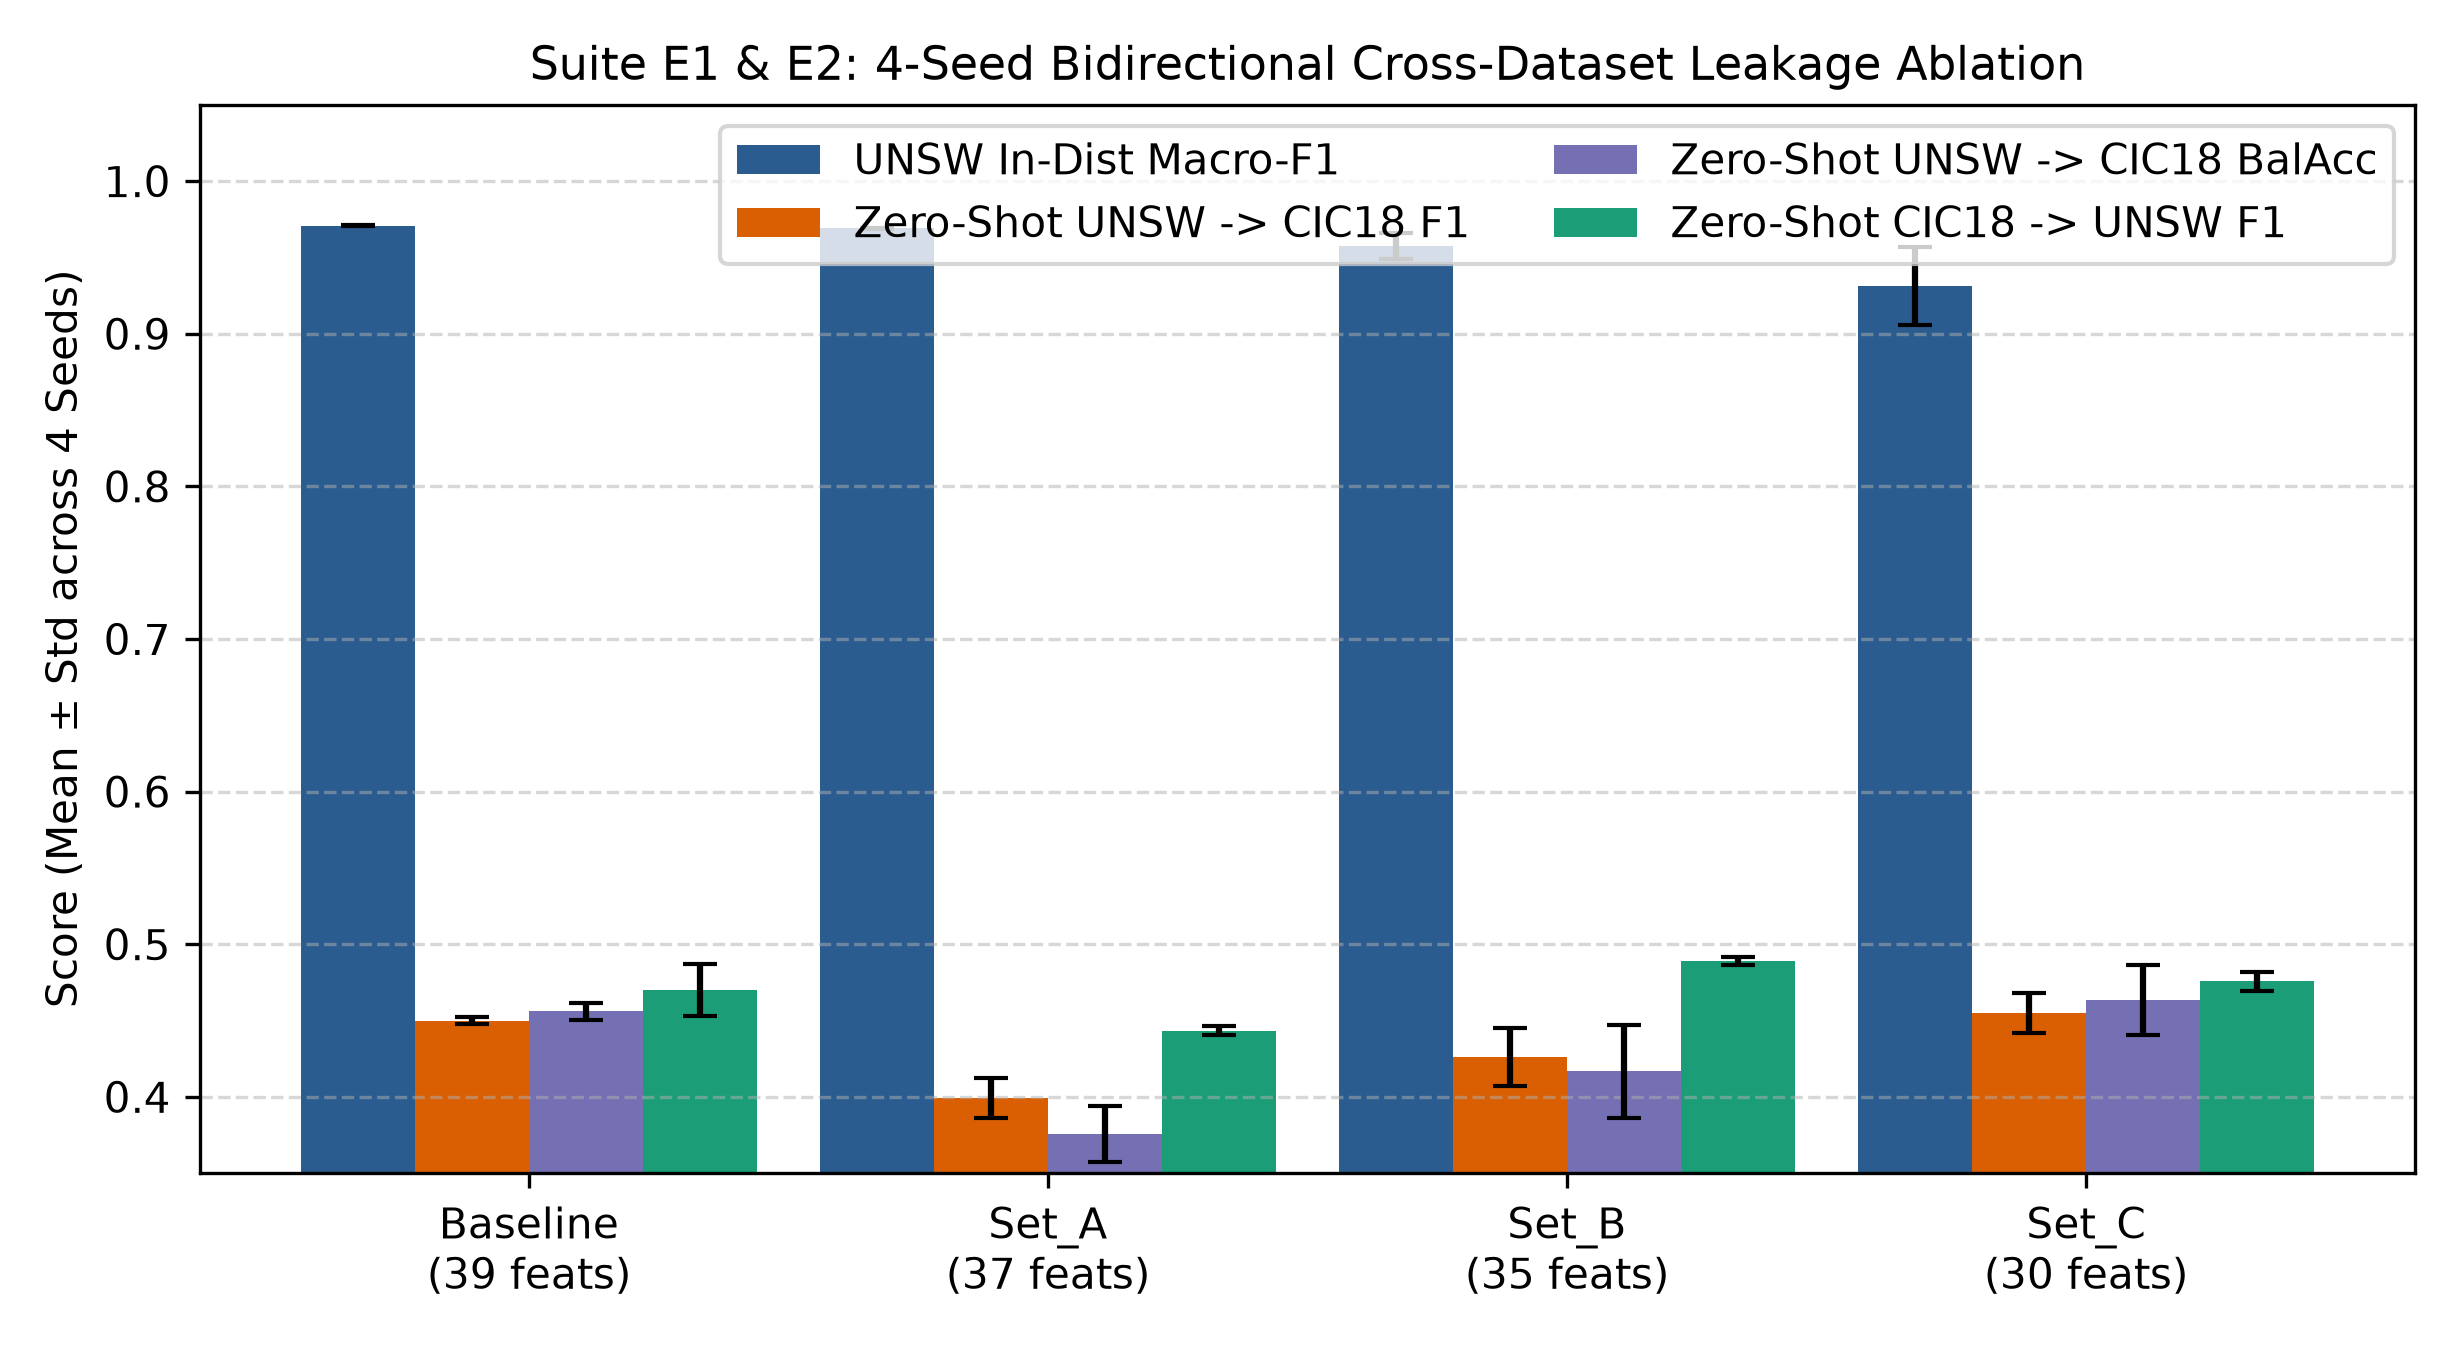
\includegraphics[width=\columnwidth]{fig1_cross_domain_ablation.png}}
\caption{Suites E1 \& E2: Four-seed bidirectional cross-dataset feature ablation (Seeds 42--45, fixed data seed 42), illustrating the `Set_A` secondary shortcut dip and bidirectional recovery at `Set_B` and `Set_C`.}
\label{fig:cross_ablation}
\end{figure}

\subsection{Suite E4: Full-Dataset Marginal Collapse vs.\ Mondrian Restoration}
Tables~\ref{tab:e4_summary} and \ref{tab:e4_per_class} evaluate Marginal SCP and Class-Conditional Mondrian MCP directly on the full `NF-UNSW-NB15-v2` known test split ($N_{\text{cal}} = 297,987$, $N_{\text{test, known}} = 297,988$).

\begin{table}[t]
\caption{Suite E4 Summary ($N_{\text{test, known}} = 297,988$): Marginal SCP vs.\ Class-Conditional Mondrian MCP at $\alpha \in \{0.10, 0.05\}$}
\begin{center}
\begin{tabular}{|l|c|c|c|c|c|r|}
\hline
\textbf{Conformal} & $\boldsymbol{\alpha}$ & \textbf{Overall} & \textbf{Worst} & \textbf{Mean Class} & \textbf{Mean} & \textbf{Empty} \\
\textbf{Method} & & \textbf{\textit{Cov (\%)}} & \textbf{\textit{Class (\%)}} & \textbf{\textit{Cov (\%)$^{\mathrm{a}}$}} & \textbf{\textit{Size}} & \textbf{\textit{Sets}} \\
\hline
Marginal SCP & 0.10 & 90.40 & 0.00 & 18.96 & 0.905 & 28,394 \\
\textbf{Mondrian MCP} & \textbf{0.10} & \textbf{90.76} & \textbf{86.94} & \textbf{90.46} & \textbf{1.133} & \textbf{14,688} \\
\hline
Marginal SCP & 0.05 & 95.01 & 4.44 & 46.94 & 0.963 & 11,093 \\
\textbf{Mondrian MCP} & \textbf{0.05} & \textbf{95.68} & \textbf{94.00} & \textbf{95.21} & \textbf{1.251} & \textbf{23} \\
\hline
\multicolumn{7}{l}{$^{\mathrm{a}}$Unweighted mean across all $K=9$ known categories on the full test split.}
\end{tabular}
\label{tab:e4_summary}
\end{center}
\end{table}

\begin{table}[t]
\caption{Suite E4 Per-Class Breakdown ($N_{\text{test, known}} = 297,988, \alpha = 0.10$, Target $90.00\%$): Calibration Stratum Sizes ($n_c$) and Empirical Coverage}
\begin{center}
\begin{tabular}{|l|r|r|c|c|r|}
\hline
\textbf{Known} & \textbf{Calib.} & \textbf{Test} & \textbf{Marginal} & \textbf{Mondrian} & \textbf{Gain} \\
\textbf{Category} & \textbf{\textit{$n_c$ ($Z_c$)$^{\mathrm{a}}$}} & \textbf{\textit{Flows}} & \textbf{\textit{SCP (\%)}} & \textbf{\textit{MCP (\%)}} & \textbf{\textit{(\% pts)}} \\
\hline
Benign & 277,597 & 276,751 & 96.07 & 90.78 & $-5.29$ \\
Exploits & 8,621 & 9,015 & 19.38 & 90.07 & $+70.69$ \\
Fuzzers & 5,636 & 5,849 & 25.78 & 91.55 & $+65.77$ \\
Reconnaissance & 3,150 & 3,250 & 0.00 & 89.97 & $+89.97$ \\
DoS & 1,134 & 1,206 & 0.41 & 91.46 & $+91.05$ \\
Generic & 1,104 & 1,133 & 21.80 & 86.94 & $+65.14$ \\
Shellcode & 421 & 424 & 0.00 & 92.22 & $+92.22$ \\
Backdoor & 170 & 180 & 7.22 & 90.00 & $+82.78$ \\
Analysis & 154 & 180 & 0.00 & 91.11 & $+91.11$ \\
\hline
\textbf{Mean ($K=9$)} & 33,109.7 & 33,109.8 & \textbf{18.96} & \textbf{90.46} & \textbf{$+71.49$} \\
\textbf{Across-Class Std} & --- & --- & \textbf{30.74} & \textbf{1.53} & \textbf{$-29.21$} \\
\hline
\multicolumn{6}{l}{$^{\mathrm{a}}$All 9 strata satisfy $n_c \ge 154 > 19$; KS fallback activations $= 0 / 9$.}
\end{tabular}
\label{tab:e4_per_class}
\end{center}
\end{table}

\textit{Interpretation and Verification:} On the full dataset where `Benign` constitutes $92.87\%$ ($276,751 / 297,988$) of known test flows, Marginal SCP satisfies the $90.00\%$ aggregate target (`90.40%` overall coverage, with `Benign` contributing $0.9287 \times 96.07\% = 89.22\%$) while **completely collapsing to `0.00%` coverage on `Analysis`, `Reconnaissance`, and `Shellcode`, and `0.41%` on `DoS`** (Fig.~\ref{fig:mondrian_cov}). Across the 8 attack categories, Marginal SCP averages just $9.32\%$ coverage (`median` $3.82\%$). Unpooled Class-Conditional Mondrian MCP lifts worst-class coverage by $+86.94$ percentage points (`0.00%` $\to$ `86.94%`), raises mean class coverage from `18.96%` to `90.46%` (compressing across-class standard deviation 20-fold from `30.74%` down to `1.53%`), and cuts empty prediction sets in half (`28,394` $\to$ `14,688` at $\alpha = 0.10$, and `11,093` $\to$ `23` at $\alpha = 0.05$).

\begin{figure}[t]
\centerline{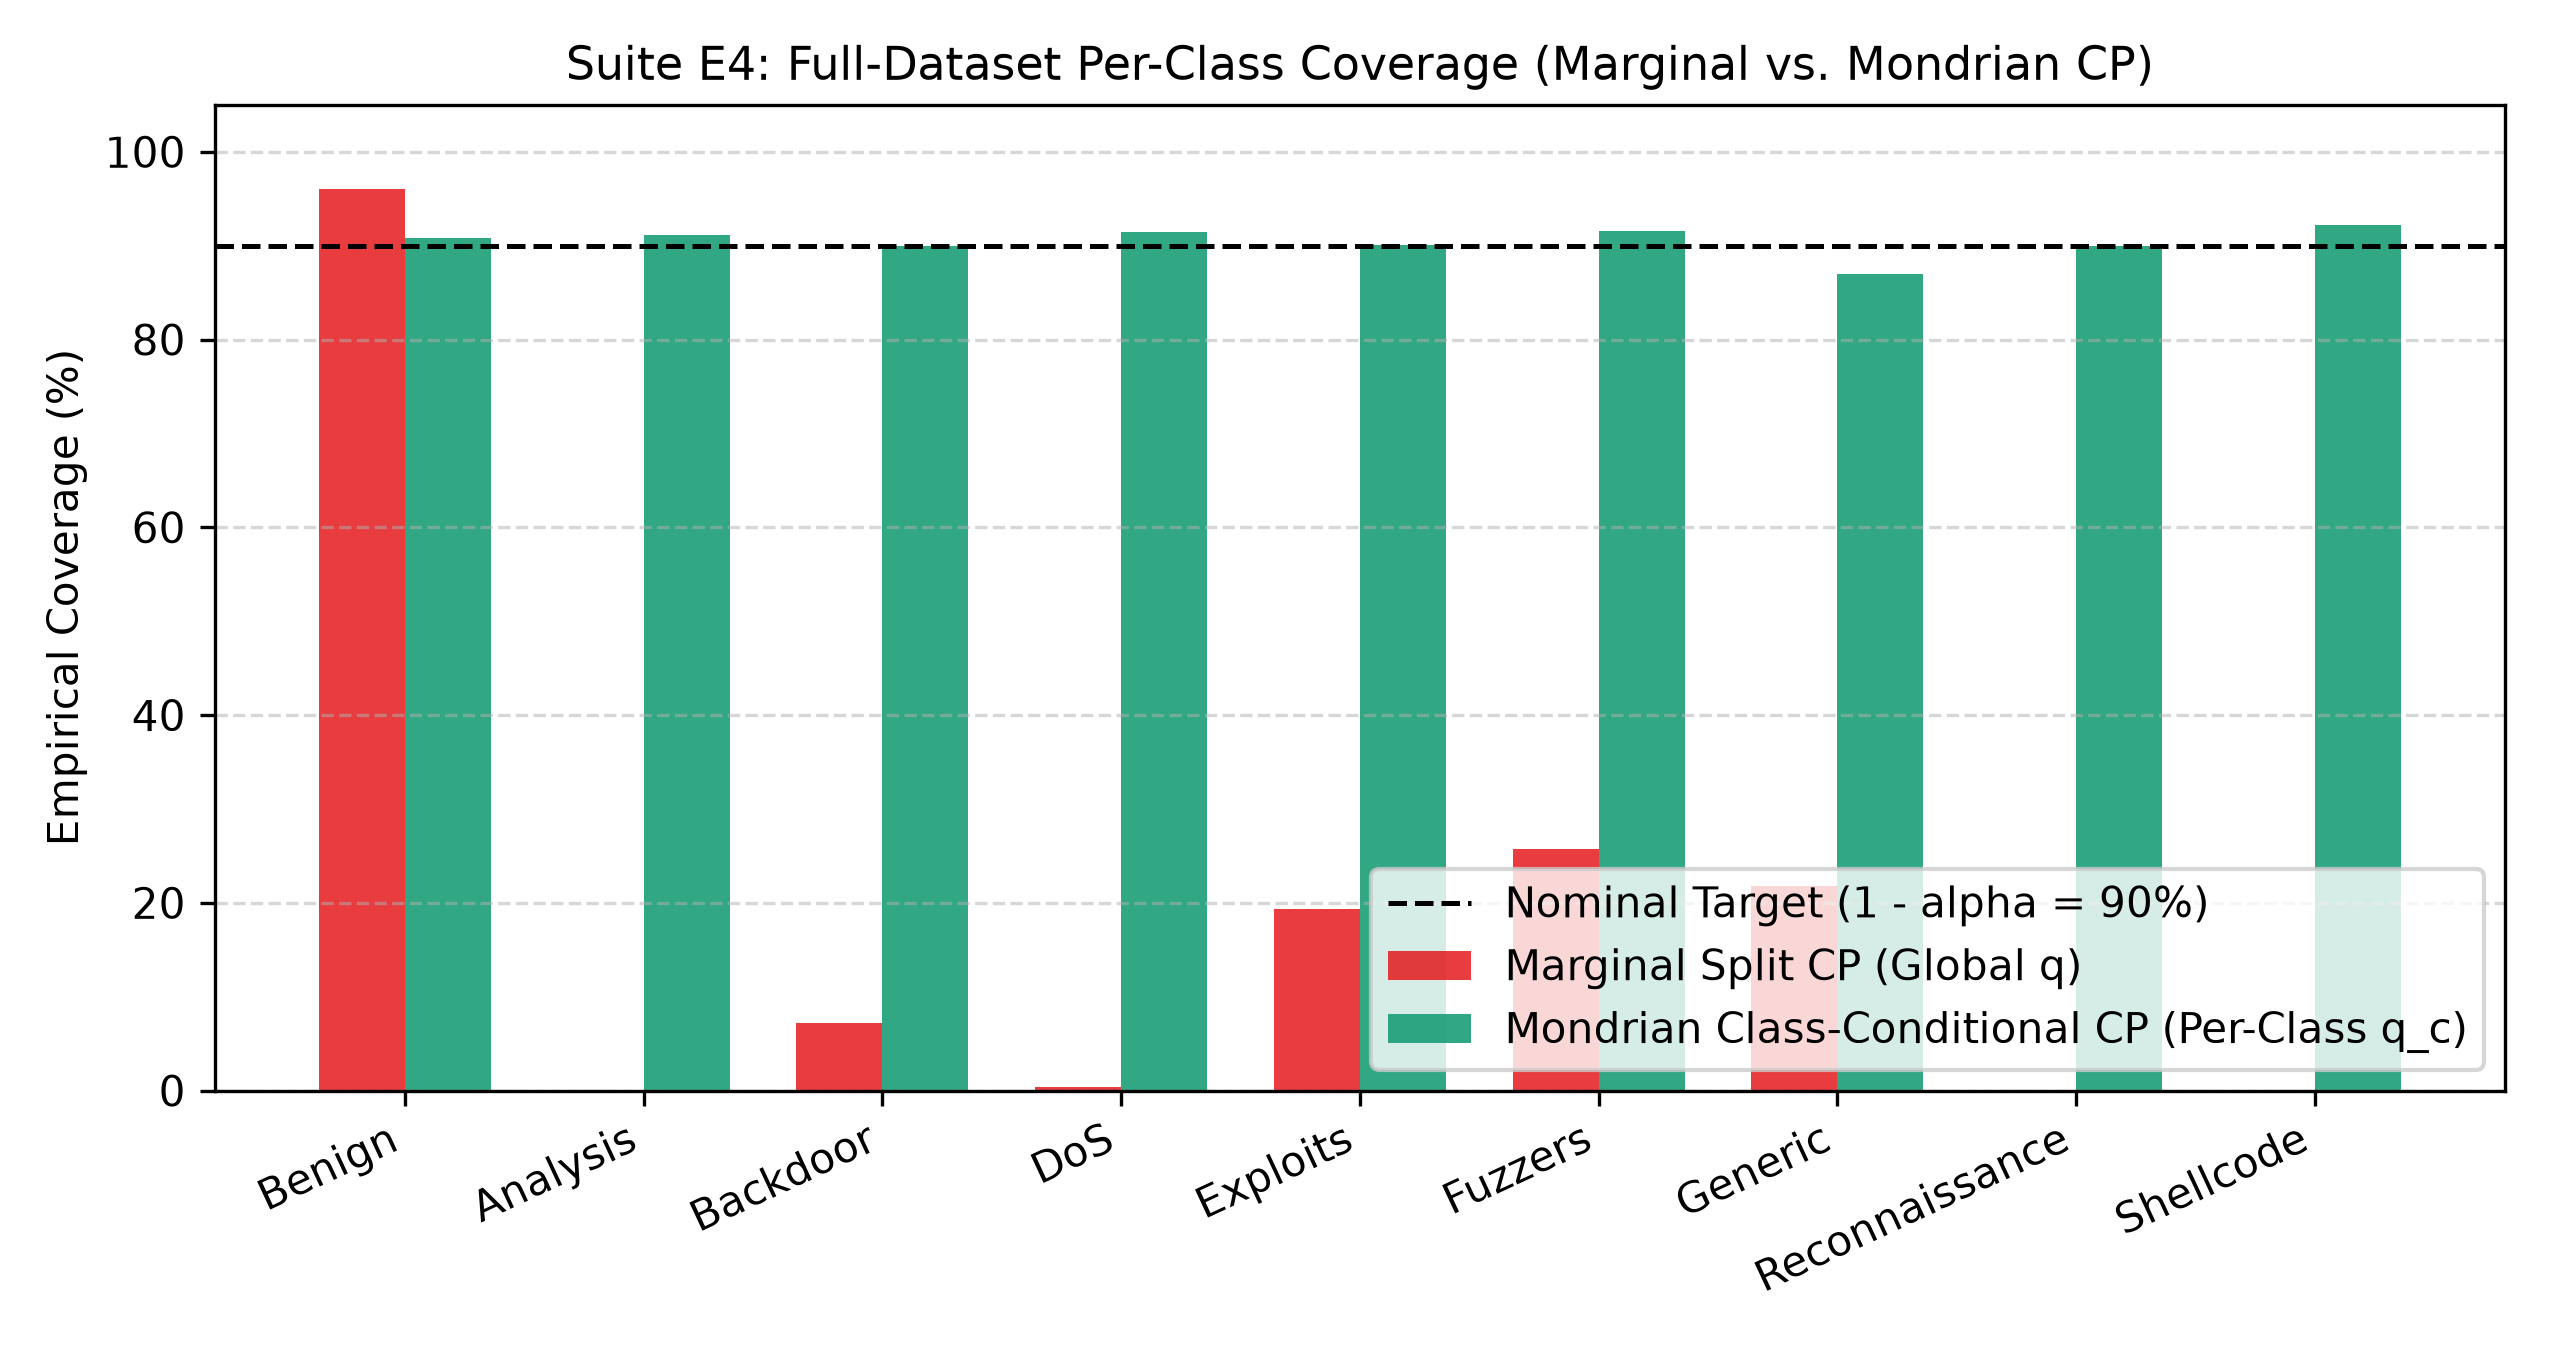
\includegraphics[width=\columnwidth]{fig2_marginal_vs_mondrian_coverage.png}}
\caption{Suite E4 ($N_{\text{test, known}} = 297,988, \alpha = 0.10$): Full-dataset empirical per-class coverage comparing Marginal SCP against unpooled Class-Conditional Mondrian MCP.}
\label{fig:mondrian_cov}
\end{figure}

\subsection{Suite E3: Full-Dataset Open-Set Recognition Audit}
Table~\ref{tab:e3_osr} evaluates open-set ranking across all $N_{\text{test}} = 298,152$ test flows ($164$ withheld `Worms` flows; unknown prevalence and random AUPR baseline $= 164 / 298,152 = 0.00055$).

\begin{table}[t]
\caption{Suite E3 ($N_{\text{test}} = 298,152, 164 \text{ Withheld Worms}, \text{Base Rate} = 0.055\%$): Unified Full-Dataset Open-Set Ranking Comparison}
\begin{center}
\begin{tabular}{|l|c|c|r|}
\hline
\textbf{Open-Set Scoring Method} & \textbf{OpenAUROC} & \textbf{OpenAUPR} & \textbf{AUPR Lift} \\
\hline
\textbf{Closed MaxProb ($1 - \max_c \hat{P}_c$)} & \textbf{0.9853} & \textbf{0.0624} & $\mathbf{113.5\times}$ \\
Euclidean OpenMax (Native Fit) & 0.9692 & 0.0141 & $25.6\times$ \\
Mahalanobis EVT + PCA Stage 2 & 0.9691 & 0.0113 & $20.5\times$ \\
True Hybrid (Maha-EVT + CP P-Val) & 0.8167 & 0.0019 & $3.5\times$ \\
Mondrian Max P-Value ($1 - \max_c p_c$) & 0.5822 & 0.0006 & $1.1\times$ \\
\hline
\end{tabular}
\label{tab:e3_osr}
\end{center}
\end{table}

\textit{Interpretation:} In continuous threshold-free ranking, `Closed_MaxProb_Baseline` (`0.9853` OpenAUROC, `0.0624` OpenAUPR) slightly outperforms `Euclidean_OpenMax_NativeFit` (`0.9692`) and `Mahalanobis_EVT_Stage2` (`0.9691`). Furthermore, standalone `Mondrian_MaxPValue_Nonconformity` ($1 - \max_c p_c(\mathbf{x})$) achieves only `0.5822` OpenAUROC because unseen `Worms` flows overlap with broad attack strata (`Exploits`, `DoS`) and therefore receive large p-values ($p_c(\mathbf{x}) > 0.10$) for multiple attack classes simultaneously. While a large maximum p-value makes $1 - \max_c p_c(\mathbf{x})$ ineffective as a standalone scalar anomaly ranker, the resulting **multi-label prediction set ($|\Gamma^\alpha(\mathbf{x})| > 1$) and narrow p-value margin ($\delta^{\text{em}}(\mathbf{x}) < 0.05$)** make Mondrian calibration highly effective as a multi-set deferral gate in Stage 6.

\subsection{Suites E5a \& E5b: Full-Scale Selective Routing and Monotone Sensitivity}
Table~\ref{tab:e5_triage} reports the full-scale selective routing telemetry on $Z_{\text{test}}$ ($N_{\text{test}} = 298,152$ flows, validation-tuned $\tau_{\text{hi}} = 0.0500$).

\begin{table*}[t]
\caption{Suite E5a (Full-Scale NF-UNSW-NB15-v2 Test Split, $N_{\text{test}} = 298,152$, Set C, Seed 42): Per-Category Recall, Mondrian Coverage ($\alpha=0.10$), OSR Rejection, and Selective Routing ($\tau_{\text{hi}}=0.0500$, Margin AURC $= 0.0231$, Gate-Consistent AURC $= 0.0124$, FAR $= 4.54\%$)}
\begin{center}
\begin{tabular}{|l|r|r|r|r|r|r|r|r|}
\hline
\textbf{Flow Category} & \textbf{Test} & \textbf{Raw Top-1} & \textbf{Empirical} & \textbf{Stage-4 OSR} & \textbf{Automated} & \textbf{Escalated} & \textbf{Automated} & \textbf{Accuracy} \\
& \textbf{\textit{Flows}} & \textbf{\textit{Recall (\%)}} & \textbf{\textit{MCP Cov (\%)}} & \textbf{\textit{Reject (\%)}} & \textbf{\textit{Share $\mathcal{A}$ (\%)}} & \textbf{\textit{Share $\mathcal{E}$ (\%)}} & \textbf{\textit{Acc in $\mathcal{A}$ (\%)}} & \textbf{\textit{Lift (\% pts)}} \\
\hline
Benign & 276,751 & 95.46 & 90.79 & 3.62 & 89.67 (248,158) & 10.33 (28,593) & 99.65 & $+4.19$ \\
Exploits & 9,015 & 66.78 & 90.06 & 3.17 & 32.00 (2,885) & 68.00 (6,130) & 89.67 & $+22.89$ \\
Fuzzers & 5,849 & 69.38 & 91.73 & 10.46 & 42.66 (2,495) & 57.34 (3,354) & 98.08 & $+28.70$ \\
Reconnaissance & 3,250 & 22.49 & 89.85 & 1.45 & 10.15 (330) & 89.85 (2,920) & 97.58 & $+75.09$ \\
DoS & 1,206 & 39.30 & 91.46 & 7.38 & 8.29 (100) & 91.71 (1,106) & 51.00 & $+11.70$ \\
Generic & 1,133 & 71.32 & 86.85 & 5.74 & 34.69 (393) & 65.31 (740) & 97.46 & $+26.14$ \\
Shellcode & 424 & 82.31 & 92.22 & 3.77 & 8.73 (37) & 91.27 (387) & 91.89 & $+9.58$ \\
Backdoor & 180 & 69.44 & 90.00 & 10.00 & 27.22 (49) & 72.78 (131) & 93.88 & $+24.44$ \\
Analysis & 180 & 13.89 & 91.11 & 6.67 & 6.67 (12) & 93.33 (168) & 83.33 & $+69.44$ \\
\hline
\textbf{Known Mean ($K=9$)} & 297,988 & \textbf{58.93} & \textbf{90.45} & \textbf{5.81} & \textbf{28.90} & \textbf{71.10} & \textbf{89.17} & \textbf{$+30.24$} \\
\hline
\textbf{Withheld Worms ($-1$)} & \textbf{164} & \textbf{31.71$^{\mathrm{a}}$} & \textbf{N/A$^{\mathrm{b}}$} & \textbf{31.71 (52)$^{\mathrm{a}}$} & \textbf{1.22 (2)$^{\mathrm{c}}$} & \textbf{98.78 (162)$^{\mathrm{d}}$} & \textbf{0.00} & \textbf{2 Leaked} \\
\hline
\multicolumn{9}{l}{$^{\mathrm{a}}$Explicit Stage-4 OSR rejection rate ($R_{\text{OSR}}(\mathbf{x}) = 1$): 52 of 164 withheld `Worms` flows ($31.71\%$).} \\
\multicolumn{9}{l}{$^{\mathrm{b}}$Conformal prediction sets $\Gamma^\alpha(\mathbf{x})$ are calibrated strictly over known classes $\mathcal{Y}_{\text{known}}$.} \\
\multicolumn{9}{l}{$^{\mathrm{c}}$Only 2 of 164 withheld `Worms` flows ($1.22\%$) bypassed both OSR and conformal deferral to enter $\mathcal{A}$.} \\
\multicolumn{9}{l}{$^{\mathrm{d}}$Total escalated `Worms` flows: 162 of 164 ($98.78\%$), comprising 52 flows ($31.71\%$) via Stage-4 OSR and 110 flows ($67.07\%$) via Stage-5/6 conformal ambiguity.}
\end{tabular}
\label{tab:e5_triage}
\end{center}
\end{table*}

\begin{figure}[t]
\centerline{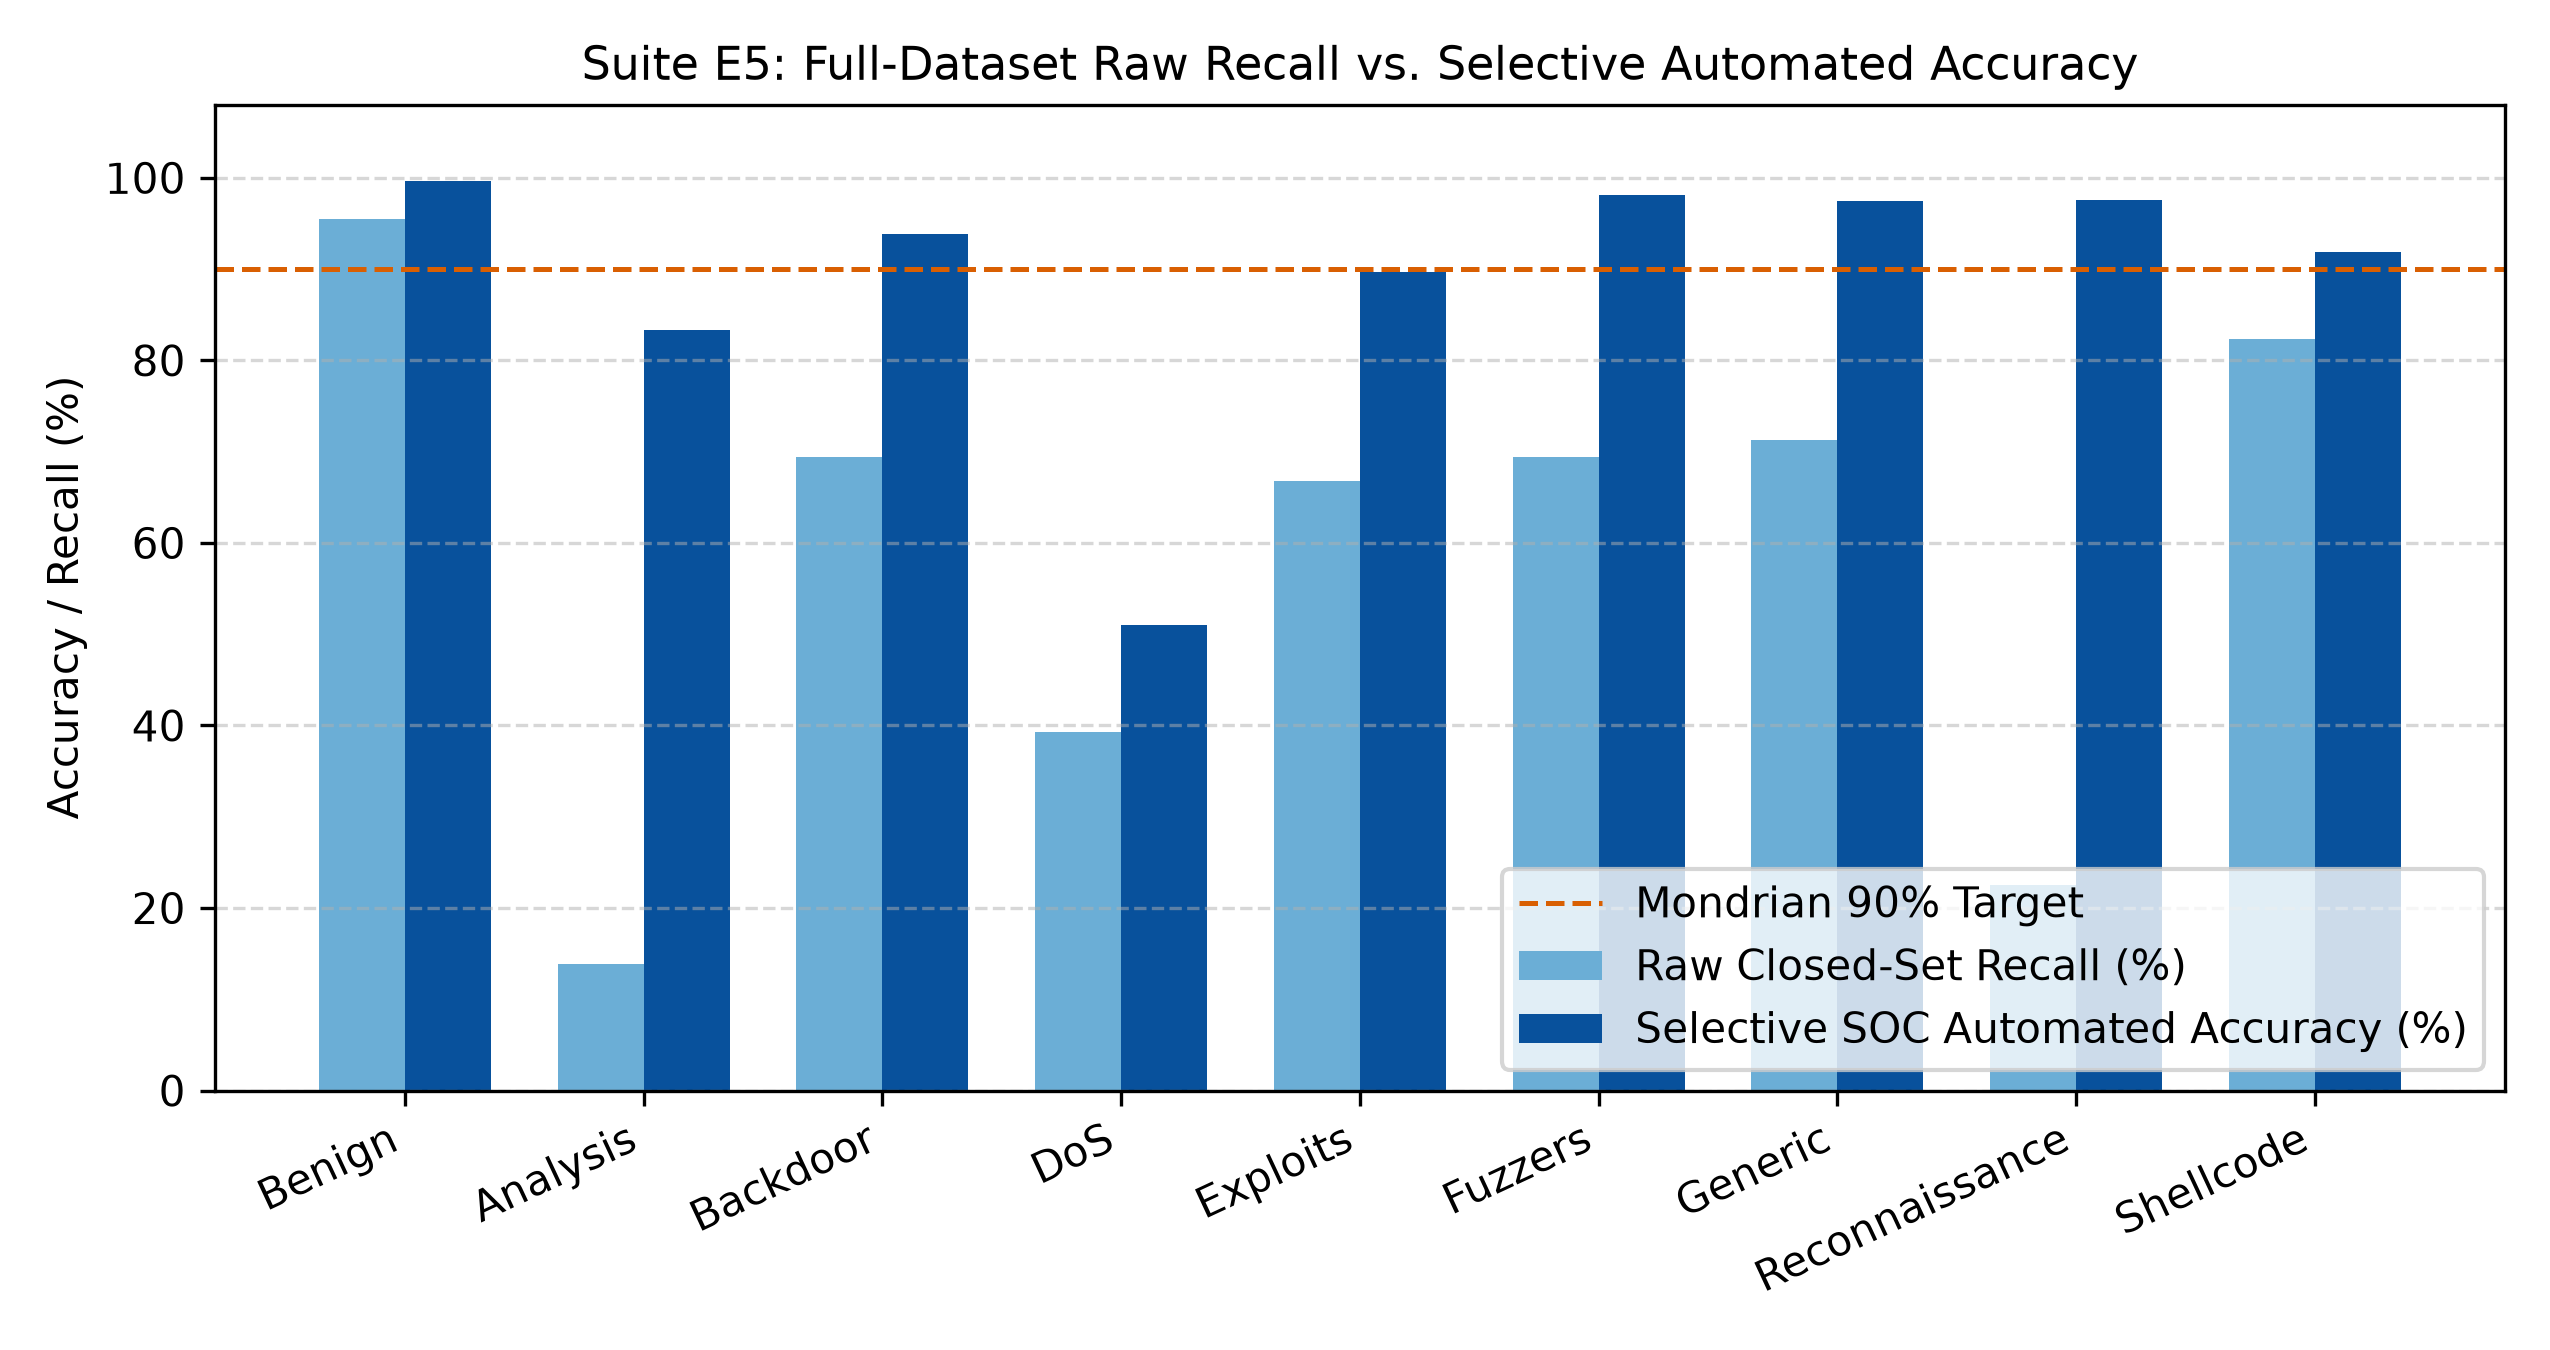
\includegraphics[width=\columnwidth]{fig3_soc_selective_triage_lift.png}}
\caption{Suite E5a ($N_{\text{test}} = 298,152$): Comparison of raw closed-set top-1 recall vs.\ selective accuracy within the gate-accepted automated subset ($\mathcal{A}$).}
\label{fig:triage_lift}
\end{figure}

\textit{Verification of Selective Routing Outcomes:}
\begin{enumerate}
    \item \textit{Overall and Attack-Only Automation Precision:} Across all $298,152$ test flows, the routing gate resolves **$85.35\%$ ($254,461$ flows)** autonomously in $\mathcal{A}$ at **$99.50\%$ overall subset accuracy**, while routing **$14.65\%$ ($43,691$ flows)** to human review in $\mathcal{E}$. Crucially, isolating the $6,303$ non-benign flows accepted into $\mathcal{A}$ confirms an **`Automated_Attack_Only_Accuracy` of $93.29\%$** ($93.32\%$ across the $6,301$ known attack flows vs.\ $59.28\%$ weighted raw attack recall, a $+34.04$ percentage-point lift). Across all 9 known categories, unweighted mean accuracy rises from $58.93\%$ raw recall to $89.17\%$ automated accuracy ($+30.24$ percentage points; Fig.~\ref{fig:triage_lift}). Furthermore, ordering prefixes by the gate-consistent priority score cuts cumulative risk by $46.3\%$, reducing `Triage_AURC` from `0.0231` to `Gate_Consistent_AURC = 0.0124`.
    \item \textit{Complementary Zero-Day Escalation ($98.78\%$):} Among the $164$ withheld `Worms` flows, Stage-4 OSR explicitly flags $52$ flows ($31.71\%$), and Stage-5/6 conformal multi-set and margin filtering catches an additional $110$ flows ($67.07\%$), escalating **$162$ of $164$ flows ($98.78\%$)** to analyst review and leaving only **$2$ flows ($1.22\%$)** autonomously misclassified.
\end{enumerate}

Finally, Table~\ref{tab:e5_evasion} verifies the binary volumetric sensitivity sweep (Suite E5b) with clean benign false-positive rates (`Benign_FPR`) reported alongside attack recall. When $5\%$ of benign training flows contain high-volume transfer profiles ($+6.0$ shift) and test attacks undergo upward volumetric shifts $+\varepsilon \cdot 6.0$ across $\mathcal{F}_{\text{vol}}$ \cite{b15,b21}, unconstrained tree recall collapses from $99.59\%$ ($\varepsilon = 0.50$) to $44.87\%$ ($\varepsilon = 0.75$) and **$15.05\%$ ($\varepsilon = 1.00$, Macro-F1 $0.4385$)**, whereas the monotone-constrained GBDT maintains **$100.00\%$ attack recall (`Macro-F1 = 0.9960`)** with a constant benign false-positive rate of $0.94\%$ (vs.\ $0.93\%$ unconstrained).

\begin{table}[t]
\caption{Suite E5b (Binary Sensitivity Sweep): Attack Recall, Macro-F1, and Benign False Positive Rate (FPR) Under Upward Volumetric Perturbation}
\begin{center}
\begin{tabular}{|c|c|c|c|c|c|c|}
\hline
\textbf{Shift} & \multicolumn{2}{|c|}{\textbf{Attack Recall (\%)}} & \multicolumn{2}{|c|}{\textbf{Binary Macro-F1}} & \multicolumn{2}{|c|}{\textbf{Benign FPR (\%)}} \\
\cline{2-7}
$\boldsymbol{\varepsilon}$ & \textbf{\textit{Uncon.}} & \textbf{\textit{Mono.}} & \textbf{\textit{Uncon.}} & \textbf{\textit{Mono.}} & \textbf{\textit{Uncon.}} & \textbf{\textit{Mono.}} \\
\hline
0.00 & 99.77 & 99.79 & 0.9947 & 0.9948 & 0.93 & 0.94 \\
0.25 & 99.97 & 100.00 & 0.9959 & 0.9960 & 0.93 & 0.94 \\
0.50 & 99.59 & 100.00 & 0.9936 & 0.9960 & 0.93 & 0.94 \\
0.75 & 44.87 & 100.00 & 0.6643 & 0.9960 & 0.93 & 0.94 \\
\textbf{1.00} & \textbf{15.05} & \textbf{100.00} & \textbf{0.4385} & \textbf{0.9960} & \textbf{0.93} & \textbf{0.94} \\
\hline
\end{tabular}
\label{tab:e5_evasion}
\end{center}
\end{table}

\section{Limitations and Future Work}
We explicitly highlight four boundaries of the present study:
\begin{enumerate}
    \item \textit{Sequential Row Order vs.\ Capture Timestamps:} Because the pre-cleaned Parquet distributions omit raw epoch timestamps, our global sequential split relies on preserved file ordering rather than verified clock cutoffs or session-grouped purging.
    \item \textit{Persistent Cross-Network Covariate Shift:} While `Set_C` recovers bidirectional transfer above `Set_A` and `Baseline`, zero-shot Balanced Accuracy across networks remains near $0.46$--$0.49$, confirming that target-domain recalibration or online adaptive conformal inference \cite{b19,b20} is required for cross-network deployment.
    \item \textit{Single Withheld Family in OSR Evaluation:} Suite E3 and Suite E5a evaluate `Worms` ($164$ flows) as the held-out attack proxy; rotating leave-one-family-out evaluations across all attack categories is an important next step.
    \item \textit{Directional Scope of Volumetric Monotonicity:} Positive monotonicity on $\mathcal{F}_{\text{vol}}$ protects specifically against upward volumetric padding into high-byte benign pockets \cite{b15}, and does not address packet-splitting or timing-based mimicry \cite{b21}.
\end{enumerate}

\section{Conclusion}
This paper presented a unified empirical audit of feature-pruned cross-dataset transfer, coupled volumetric monotonicity, calibration-fitted open-set recognition, class-conditional Mondrian conformal prediction, and validation-tuned selective routing across `NF-UNSW-NB15-v2` and `NF-CSE-CIC-IDS2018-v2`. Our results reveal a non-monotonic shortcut cascade when pruning header groups, prove that standard marginal conformal prediction suffers a total $0.00\%$ coverage collapse on three minority attack categories under full-scale base-rate skew that unpooled Mondrian calibration restores to $86.94\%$--$92.22\%$, and demonstrate that combining calibration-fitted OSR with conformal multi-set deferral escalates $98.78\%$ of unseen `Worms` flows while automating $85.35\%$ of network traffic at $99.50\%$ overall ($93.29\%$ attack-only) accuracy.

\begin{thebibliography}{00}
\bibitem{b1} D. Arp, E. Quiring, F. Pendlebury, A. Warnecke, F. Pierazzi, C. Wressnegger, L. Cavallaro, and K. Rieck, ``Dos and don'ts of machine learning in computer security,'' in \textit{Proc. 31st USENIX Security Symp.}, Boston, MA, USA, Aug. 2022, pp. 3971--3988.
\bibitem{b2} M. Sarhan, S. Layeghy, and M. Portmann, ``Evaluating standard feature sets towards increased generalisability and explainability of ML-based network intrusion detection,'' \textit{Big Data Res.}, vol. 30, Nov. 2022, Art. no. 100359.
\bibitem{b3} G. Engelen, V. Rimmer, and W. Joosen, ``Troubleshooting an intrusion detection dataset: The CICIDS2017 case study,'' in \textit{Proc. IEEE Security and Privacy Workshops (SPW)}, San Francisco, CA, USA, May 2021, pp. 7--12.
\bibitem{b4} A. Rosay, E. Cheval, F. Carlier, and P. Leroux, ``Network intrusion detection: A comprehensive analysis of CIC-IDS2017,'' in \textit{Proc. 8th Int. Conf. Inf. Syst. Security and Privacy (ICISSP)}, Feb. 2022, pp. 25--36.
\bibitem{b5} M. Lanvin, P.-F. Gimenez, Y. Han, F. Majorczyk, L. M\'e, and E. Totel, ``Errors in the CICIDS2017 dataset and the significant differences in detection performances it makes,'' in \textit{Proc. Int. Conf. Risks and Security of Internet and Systems (CRiSIS)}, 2023, pp. 18--33.
\bibitem{b6} M. Cantone, C. Marrocco, and A. Bria, ``Machine learning in network intrusion detection: A cross-dataset generalization study,'' \textit{IEEE Access}, vol. 12, pp. 144489--144508, 2024, doi: 10.1109/ACCESS.2024.3472907.
\bibitem{b7} C. K\i l\i \c{c} and G. \c{S}eng\"ul, ``SHAP-guided feature selection for cross-dataset generalization in network intrusion detection systems,'' \textit{IEEE Access}, vol. 14, pp. 90926--90936, 2026, doi: 10.1109/ACCESS.2026.3703481.
\bibitem{b8} P. Toccaceli and A. Gammerman, ``Combination of inductive Mondrian conformal predictors,'' \textit{Mach. Learn.}, vol. 108, no. 3, pp. 489--510, Mar. 2019, doi: 10.1007/s10994-018-5754-9.
\bibitem{b9} A. Bendale and T. E. Boult, ``Towards open set deep networks,'' in \textit{Proc. IEEE Conf. Comput. Vis. Pattern Recognit. (CVPR)}, Las Vegas, NV, USA, Jun. 2016, pp. 1563--1572.
\bibitem{b10} T. T. Nguyen and M. Park, ``MaGOS-IDS: A Mahalanobis-enhanced OpenMax method for graph neural network-based intrusion detection,'' \textit{Electronics}, vol. 15, no. 16, Aug. 2026, Art. no. 3667, doi: 10.3390/electronics15163667.
\bibitem{b11} H. Linusson, U. Johansson, H. Bostr\"om, and T. L\"ofstr\"om, ``Classification with reject option using conformal prediction,'' in \textit{Proc. Pacific-Asia Conf. Knowl. Discovery and Data Mining (PAKDD)}, Melbourne, VIC, Australia, Jun. 2018, pp. 94--105.
\bibitem{b12} F. \c{S}ahin and N. S. Mert, ``Dual-threshold conformal deferral for trustworthy security alert triage,'' \textit{Electronics}, vol. 15, no. 18, Sep. 2026, Art. no. 4084, doi: 10.3390/electronics15184084.
\bibitem{b13} A. Moccardi, A. Amato, R. C. Ghosh, and E. Cirillo, ``CRISP: Conformal resilient intrusion detection with selective prediction,'' in \textit{Proc. 6th Int. Conf. Mach. Learn. and Intell. Syst. Eng. (MLISE)}, 2026, pp. 63--72.
\bibitem{b14} L. Grinsztajn, E. Oyallon, and G. Varoquaux, ``Why do tree-based models still outperform deep learning on typical tabular data?'' in \textit{Advances in Neural Information Processing Systems (NeurIPS)}, vol. 35, 2022, pp. 507--520.
\bibitem{b15} M. Theodorides, S. Afroz, and D. Wagner, ``Adversarially robust malware detection using monotonic classification,'' in \textit{Proc. 4th ACM Int. Workshop Security and Privacy Analytics (IWSPA)}, Tempe, AZ, USA, Mar. 2018, pp. 47--54.
\bibitem{b16} V. Vovk, A. Gammerman, and G. Shafer, \textit{Algorithmic Learning in a Random World}. New York, NY, USA: Springer, 2005.
\bibitem{b17} U. Johansson, E. Ahlberg, H. Bostr\"om, L. Carlsson, H. Linusson, and C. S\"onstr\"od, ``Handling small calibration sets in Mondrian inductive conformal regressors,'' in \textit{Proc. Int. Symp. Statist. Learn. and Data Sci. (SLDS)}, 2015, pp. 271--280.
\bibitem{b18} T. Ding, A. Angelopoulos, S. Bates, M. Jordan, and R. J. Tibshirani, ``Class-conditional conformal prediction with many classes,'' in \textit{Advances in Neural Information Processing Systems (NeurIPS)}, vol. 36, 2023.
\bibitem{b19} R. F. Barber, E. J. Cand\`es, A. Ramdas, and R. J. Tibshirani, ``Conformal prediction beyond exchangeability,'' \textit{Ann. Statist.}, vol. 51, no. 2, pp. 816--845, Apr. 2023, doi: 10.1214/23-AOS2276.
\bibitem{b20} I. Gibbs and E. J. Cand\`es, ``Conformal inference for online prediction with arbitrary distribution shifts,'' \textit{J. Mach. Learn. Res.}, vol. 25, no. 162, pp. 1--36, 2024.
\bibitem{b21} V. Kumar, K. Kumar, and M. Singh, ``NIDS-CBAD: Detecting adversarial attacks in network intrusion detection systems using domain constraints,'' \textit{Int. J. Mach. Learn. Cybern.}, vol. 16, pp. 4213--4234, 2025, doi: 10.1007/s13042-024-02506-8.
\end{thebibliography}

\end{document}
